\subsection{Placa base}\label{sec:motherboard}

Una vegada escollits dos processadors com a contrincants, hem començat a mirar quines plaques bases hi havia al mercat. Primerament, les hem anat buscant de manera individual i les que hem seleccionat es poden veure a la taula següent:

\begin{table}[H]
\begin{adjustwidth}{-.5in}{-.5in}  
    \begin{center}
    \centering
    \scalebox{1.0}{
\begin{tabular}{l||c|c|c|c|c|c}
    \hline
Placa mare & \begin{tabular}[c]{@{}c@{}}Nuclis \\ Màx.\end{tabular} & \begin{tabular}[c]{@{}c@{}}Storage \\ Speed\end{tabular} & \begin{tabular}[c]{@{}c@{}}DIMS \\ Màx.\end{tabular} & \begin{tabular}[c]{@{}c@{}}USB \\ 3.0\end{tabular} & PCIe 4.0 & \begin{tabular}[c]{@{}c@{}}Preu \\ (Euros)\end{tabular} \\ \hline \hline
\rowcolor[HTML]{EFEFEF}
H12DSU-iN \cite{mother1} & 64 & 6 Gbps & 32 & 5 & 1x16, 1x32, 1x40 & Coming soon \\ 
H12DST-B \cite{mother2} & 64 & 6 Gbps & 16 & 2 & 3x16, 1x24 & - \\ 
\rowcolor[HTML]{EFEFEF}
H12SSW-NT \cite{mother3} & 64 & 6 Gbps & 8 & 7 & 1x16, 1x32 & 1356.53 \cite{mother3_preu}\\
H12SSW-iN \cite{mother4} & 64 & 6 Gbps & 8 & 7 & 2x32 & - \\
\rowcolor[HTML]{EFEFEF}
H12SST-PS \cite{mother5} & 64 & 6 Gbps & 8 & 2 & 3x16 & 3959.86 \cite{mother5_preu}\\ \hline 
\end{tabular}
}
    \caption{Comparació inicial de plaques base.}
    \label{tab:_placa_base_cmp}
    \end{center}
    \end{adjustwidth}
\end{table}

Com es pot veure, les diferències principals són el número de DIMS de memòria i els PCI-Express. No obstant, una vegada fetes les comparacions inicials, ens hem adonat que per algunes d'elles era excessivament complicat trobar el preu. Per exemple, els llocs on trobàvem els preus no eren els mateixos on trobàvem les especificacions, per tant en algunes plaques no estem segurs de que els preus siguin del tot realistes.

Buscant els preus hem trobat una altra web \cite{webnodes} que ens permet crear un node seleccionant nosaltres els seus components. Hem vist que els tipus de node es diferencien inicialment entre aquells amb GPU i aquells sense GPU. Dins d'aquests dos grups trobem també els dual-socket i els single-socket.

Com que el processador \textit{AMD EPYC 7702P} té 64 nuclis i l'\textit{AMD EPYC Rome 7502P} en té 32, hem decidit plantejar-nos les opcions de nodes dual-socket amb dos processadors \textit{7502P} i nodes single-socket amb el processador \textit{7702P}. En cas d'escollir un node amb suport per GPU, ocuparem 2U en compte d'una de sola. En el cas dels nodes amb dual-socket, es poden suportar fins a 8 GPUs mentre que amb els single-socket només la meitat, 4.

\begin{figure}[H]
    \centering
    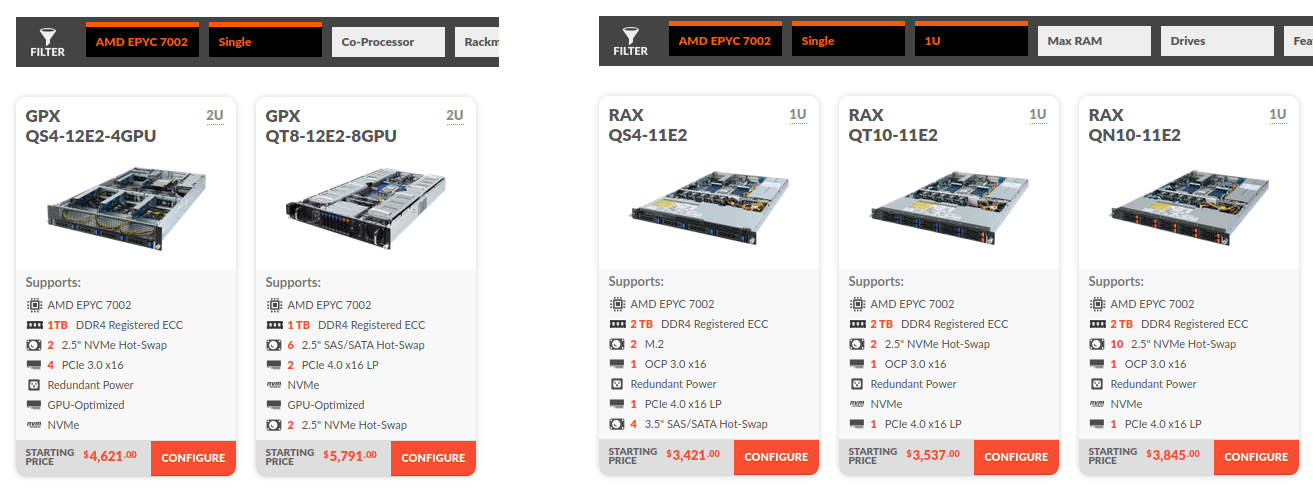
\includegraphics[width=\textwidth]{img/webnodes.png}
    \caption{Exemple de nodes que podem trobar a la web. A l'esquerra amb GPUs i a la dreta sense. Tots single-socket.}
\end{figure}

En la taula \ref{tab_web_plaques_cmp} es veuen aquestes possibles combinacions. En el cas d'utilitzar un node amb GPUs no s'ha inclòs el preu de la pròpia GPU, ja que això dependrà de quina escollim més endavant. Per la mateixa raó, tampoc s'han exposat els GFflops de les versions amb GPU. En aquests preus tampoc s'inclouen els costos de les memòries i les targetes de xarxa.

\begin{table}[h]
\begin{adjustwidth}{-.5in}{-.5in}  
    \begin{center}
    \centering
    \scalebox{1.0}{
\begin{tabular}{l||c|c|c|c|c|c}
    \hline
Configuració & Nuclis & \begin{tabular}[c]{@{}c@{}}GFlops \\ CPU\end{tabular} & GPUs & Us & \begin{tabular}[c]{@{}c@{}}Preu \\ (Euros)\end{tabular} & \begin{tabular}[c]{@{}c@{}}GFlops/ \\ Euros\end{tabular} \\ \hline \hline
 &  &  & \cellcolor[HTML]{EFEFEF}- & \cellcolor[HTML]{EFEFEF}1 & \cellcolor[HTML]{EFEFEF}9393 & \cellcolor[HTML]{EFEFEF}0.256 \\  
\multirow{-2}{*}{\begin{tabular}[l]{@{}l@{}}Dual amb AMD\\ EPYC Rome 7502P \cite{dualnogpu}\cite{dualgpu}\end{tabular}} & \multirow{-2}{*}{128} & \multirow{-2}{*}{2560} & 8 & 2 & 12266 & - \\ \hline
 &  &  & \cellcolor[HTML]{EFEFEF}- & \cellcolor[HTML]{EFEFEF}1 & \cellcolor[HTML]{EFEFEF}7542 & \cellcolor[HTML]{EFEFEF}0.251 \\  
\multirow{-2}{*}{\begin{tabular}[l]{@{}l@{}}Single amb AMB\\ EPYC 7702P \cite{singlenogpu}\cite{singlegpu}\end{tabular}} & \multirow{-2}{*}{128} & \multirow{-2}{*}{2048} & 4 & 2 & 9461 & - \\ \hline
\rowcolor[HTML]{EFEFEF}
\end{tabular}
}
    \caption{Comparació entre les diferents configuracions dels nodes. \textit{Nota: Els preus de les referències poden no ser exactament iguals que els de la taula, ja que s'han descomptat alguns preus com el de la memòria o disc}}
    \label{tab:web_plaques_cmp}
    \end{center}
    \end{adjustwidth}
\end{table}

Veiem que tot i que la versió amb dual-socket ens proporciona més GFlops, l'eficiència GFlops/dòllar és millor per la versió amb single-socket. Per tant, en aquest punt encara no podem decantar-nos per cap de les dues. Una vegada haguem considerat quines GPUs utilitzem, quina xarxa tenim, etc., podrem valorar si tenim suficient pressupost com per escollir la opció amb més GFlops. A més, quan les GPUs entrin en joc també s'haurà de tenir en compte que amb l'opció dual-socket en podem posar-ne el doble per cada node.

